\section{Video Player}
\subsection{Ziel}
In einem ersten Schritt, noch vor der Realisierung des Fahrsimulator wird ein Video-Player ralisiert. Das Ziel des Video-Players ist es eine Verbindung zwischen dem Cockpit und unserem Programm herzustellen und diese zu Testen. Bei der Betätigung des Gaspedals im Cockpit soll das aufgenommene Video schneller abgespielt werden. Bei der Betätigung des Bremspedals dementsprechend langsamer. Der Video-Player soll so gegliedert werden, damit Komponenten davon auch im Fahrsimulator wiederverwendet werden können. Zudem ist die Darstellung einer Tunneleinfahrt mit den richtigen Lichtverhältnissen in einer 3D-Umgebung sehr schwierig. Eine gute Alternative bietet ein aufgenommenes Video einer Tunneleinfahrt. Die ETH-Zürich besitzt bereits Videos die sich dafür eigenen. Um Experimente mit diesen Videos durchführen zu können, müssen Manipulationen die der Proband im Cockpit mach mit dem entsprechenden Zeitpunkt im Video abgespeichert werden. Dies dient zur späteren Auswertung der Experimente. 
\\
\subsection{Systembeschreibung}

% Bild für Systembeschreibung des Video Players
\begin{figure}[h]
\centering 
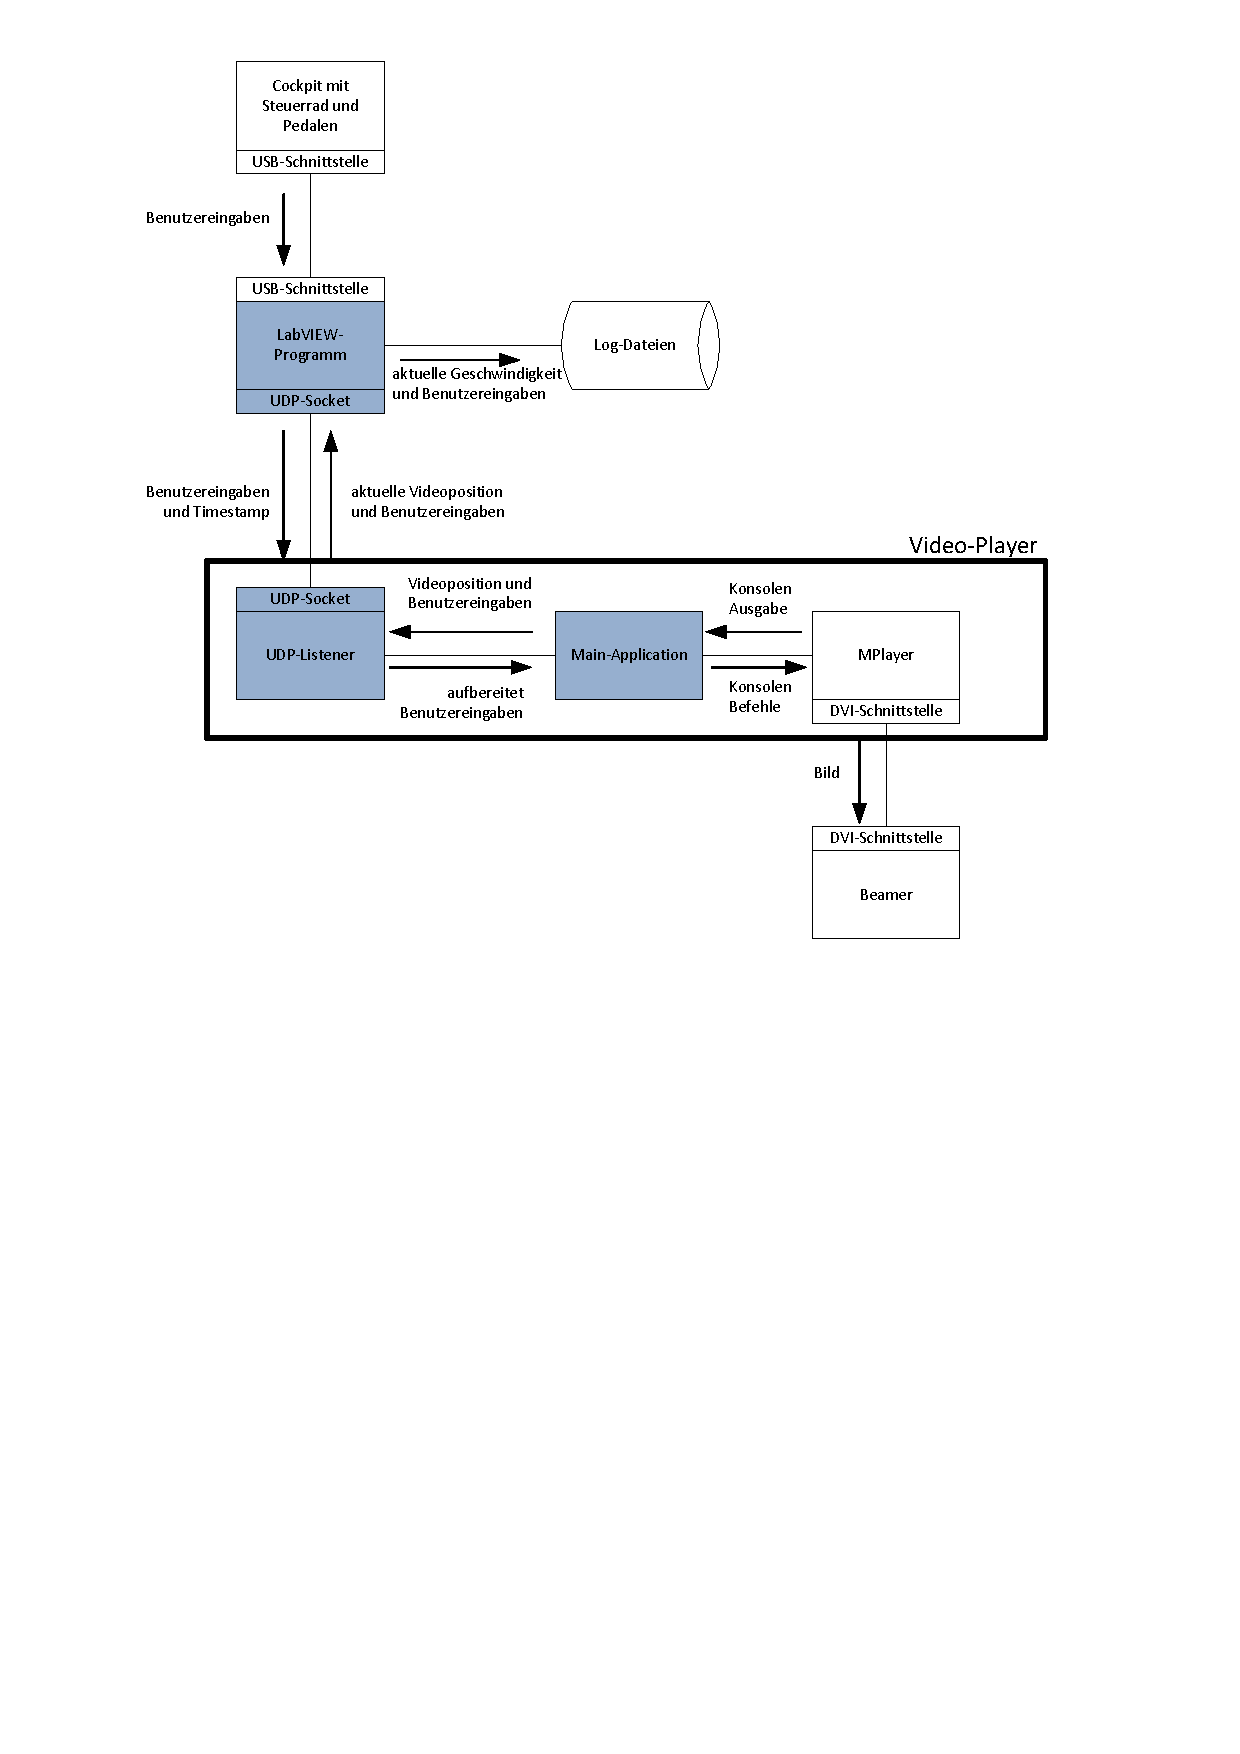
\includegraphics[width=0.8\linewidth]{src/Systembeschreibung_VideoPlayer.pdf}
\caption{Systembeschreibung Video-Player} % Titel der Grafik
\label{Systembeschreibung Video-Player} % Labelname
\end{figure}
Um einzelne Komponenten des Video-Player wiederverwenden zu können, wird das System möglichst gleich wie das des Fahrsimulators aufgebaut. Dieser Aufbau wird anhand der Abbildung \ref{Systembeschreibung Video-Player} illustriert. Blau markiert sind eingens entwickelte Komponenten des Videoplayers. Die Eingaben im Cockpit werden von einem LabVIEW-Programm über eine USB-Schnittstelle eingelesen. Die eingelesenen Parameter werden, zusammen mit einem Timestamp, von LabVIEW in ein UDP-Packet verpackt und über ein UDP-Socket gesendet. Das UDP-Packet wird von einem UDP-Listener empfangen und gelesen. Dieser speichert die empfangenen Parameter ab und hält sie für das Hauptprogramm bereit. Das Hauptprogramm (Main Application) liest die gespeicherten Parameter aus und interpretiert diese. Das Hauptprogramm steuert die Geschwindigkeit des Videos über Konsolen-Befehle. Der MPlayer, der für das abspielen der Videos verwendet wird, lässt durch die Konsolenbefehle das Video schneller oder langsamer laufen. Über die Konsole gibt der MPlayer die aktuelle Position des Videos aus. Diese Positionsdaten werden vom Hauptprogramm empfangen, mit Benutzereingaben ergänzt und an den UDP-Listener weitergeleitet. Dieser verpackt alle Daten vom Hauptprogramm in ein UDP-Packet und sendet es an das LabVIEW-Programm. Das LabVIEW-Programm benötigt einen zweiten UDP-Socket um Daten zu empfangen. Die empfangenen Daten vom UDP-Listener werden sofort in ein Log-File gespeichert, damit diese für eine Auswertungen zur Verfügung stehen. 

\subsection{Realisierung}
Bei der Realisierung des Vidoe-Players wird der Fokus vorallem auf die Entwicklung der LabVIEW Schnittstelle mit unserem Programm gelegt. Darum wird dieser Schritt der Realisierung nachfolgend ausführlich erklährt. Diese Schnittstelle wird auch für den Fahrsimulator selbst verwendet. Die Realisierung des Video-Players wird ebenfalls erläutert. 
\subsubsection{LabVIEW Schnittstelle}
Die Realisierung der LabVIEW Schnittstelle wird in zwei Teile unterteilt. Der erste Teil dient dazu die Eingaben, die im Cockpit gemacht werden, einzulesen und an den UDP-Listener zu senden. Der zweite Teil befasst sich mit dem Empfangen von Daten, die vom UDP-Listener gesendet werden und dessen speicherung in ein LogFile. 

% LabVIEW Screenshot um Daten zu senden
%\begin{figure}[h]
%\centering 
%\includegraphics[width=0.8\linewidth]{src/labview_screenshot_daten_senden.pdf}
%\caption{LabVIEW Screenshot um Daten zu senden} % Titel der Grafik
%\label{labview_screenshot_daten_senden} % Labelname
%\end{figure}
Die Abbildung \ref{labview_screenshot_daten_senden} illustriert den Aufbau des LabVIEW-Programms um die Cockpitparameter zu lesen und über einen UDP-Socket zu senden. an die "Remot Address" wird das UDP-Packet gesendet. Da sich der UPD-Listener zur Zeit noch auf dem selben Rechner wie dieses Programm befindet, wählen wir hierfür die localhost-Adresse. Für den "Romote Port" wählen wir einen freien Port. Zusammen mit dem "Local Port" der uns eine Verbindungs-ID generiert ist unsere Konfiguration für den UDP-Socket vollständig. Um die Komponenten im Cockpit ansprechen zu können muss lediglich die Richtige "Device ID" gewählt werden. Die anderen Komponenten, die sich in der grauenn Box befinden werden immer wieder ausgeführt, da die graue Box eine Schleife darstellt. Die Schleife wird alle 0.01 Sekunden wiederholt. Dieser Wert wird im "Time Delay" Element konfiguriert. \\
Aus dem Cockpit werden die Werte der x- und y-Achse ausgelesen. Auf der y-Achse wird die beiden Pedalen, Gas- und Bremspedal, abgebildet. Ein positiver Wert auf der y-Achse quantiviziert hierbei ein Druck auf das Gaspedal und ein negativer Wert das Drücken des Bremspedals. Die intensität beider Pedalen wird im positiven durch 32767 und im negativen duchr 32768 ganzzahlige Werte quantiviziert. Ein voll gedrücktes Gaspedal entspricht also dem Wert 32767 auf der y-Achse und ein voll gedrücktes Bremspedal entspricht dem Wert -32768. Die x-Achse quantifiziert den Einschlagswinkel des Steuerrades. Dieser Wert wird ebenfalls ausgelesen ist aber im Video-Player nicht relevant. Die Werte werden zusammen mit einem vom Uhrensymbol kommenden Timestamp durch ein Semikolon getrennt in das UDP-Packet gepackt und dann, ausserhalb der Schleife, gesendet.


% LabVIEW Screenshot um Daten zu empfangen
%\begin{figure}[h]
%\centering 
%\includegraphics[width=0.8\linewidth]{src/labview_screenshot_daten_empfangen.pdf}
%\caption{LabVIEW Screenshot um Daten zu empfangen} % Titel der Grafik
%\label{labview_screenshot_daten_emfpangen} % Labelname
%\end{figure}
Die Abbildung \ref{labview_screenshot_daten_senden} illustriert den Aufbau des LabVIEW-Programms um die Daten zu empfangen und in ein Log-File zu speichern. 

\begin{figure}[h]
\centering 
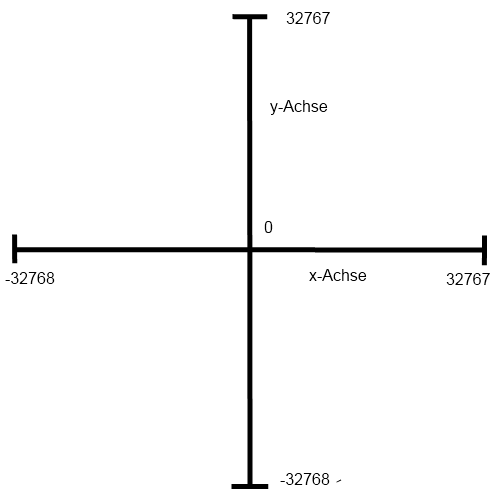
\includegraphics[width=0.5\linewidth]{src/koordinatensystem.png}
\caption{Koordinatensystem} % Titel der Grafik
\label{Koordinatensystem2} % Labelname
\end{figure}

Diese beiden Werte werden im LabVIEW-Programm in ein UDP-Packet verpackt und über das Netzwerk gesendet. Der UDP-Listener empfängt diese Packete und speichert die x und y-Werte separat ab. Das Hauptprogramm greift auf diese Werte zu, interpretiert diese und Steuert das Video.\\
Der Video Player wird in einem eigenen Prozess gestartet. 
% Code
%sprintf(arguments, " --extraintf telnet --telnet-port %d --telnet-password %s", vlcPort, vlcPassword);
%CreateProcessA(vlcExe, arguments, 0, 0, FALSE, 0, 0, 0, LPSTARTUPINFOA(&si), &pi);
%Code ende
Die erste Zeile speichert alle Argumente in der Variabel "arguments". Durch die mitgegebenen Argumente wird der Video Player mit einem extra Telnetinterface gestartet.  Das Telnetinterface hört auf den angegebenen Port. In der zweiten Zeile wird der Prozess erstellt und in diesem Prozess wird der Video Player ausgeführt. 
Nun können Manipulationsbefehle über den "send" Befehl an den mPlayer geschickt werden. Hier ein Beispiel eines solchen Befehls.
%Code
%send(socketId, message, strlen(message)
%CodeEnde
Der send-Befehl verlangt eine Socket-Id, die Nachricht,  in unserem Fall den Befehl, und die Länge der Nachricht. Das Hauptprogramm liest nun aus dem UDP-Listener den y-Wert der empfangenen Packete aus. Liegt dieser Wert über 20000 ist das Gaspedal mindestens zu zwei drittel gedrückt. Dann sendet das Hauptprogramm über die Telnetverbindung den Befehl an den Video Player die Geschwindigketi des Videos zu erhöhen. Fall der Wert unter -20000 liegt, ist das Bremspedal mindestens zu zwei drittel gedrückt. Das Hauptprogramm veranlasst den Videoplayer die Geschwindigkeit des Videos u reduzieren. 